% !TEX root = main.tex

\section{数据链路层}
数据链路层把\textemph{数据帧(frame)},从一个节点通过链路\footnote{链路即连接相邻节点的通道,包括有线链路、无线链路、局域网等}(直连网络/\textemph{物理网络})传给\textemph{相邻}另一个节点(主机或路由器)。

\bigskip
数据链路层的功能如下:
\begin{partlist}
	\item \underline{成帧}(framing)
	\item \underline{差错检测}(error detect):比特错,纠错
	\item \underline{差错控制}(error control):丢包、重复、错序、流控制(flow control)
	\item \underline{介质访问控制}(medium access control):多路访问,碰撞(collision)
\end{partlist}

\bigskip
针对点对点和多路访问网络又分别制定了两个子层:
\begin{itemize}
	\item \underline{逻辑链路控制(Logic Link Control, LLC)子层}:提供可靠数据传输
	\begin{itemize}
		\item LLC1提供\textemph{无确认无连接}服务
		\item LLC2提供\textemph{有确认面向连接}的服务,实现滑动窗口协议
		\item LLC3提供\textemph{有确认无连接}的服务
	\end{itemize}
	\item \underline{介质访问控制(Media Access Control, MAC)子层}:专门用来处理多路访问网络中的冲突(点对点网络没有冲突就不用)
\end{itemize}

注意数据链路层、网络层错了就错了,不提供纠正服务,由上层纠正。
链路层在\textemph{网络接口卡(network interface card, NIC)及其驱动程序}上实现,路由器在\textemph{接口模块}上实现。

\begin{figure}[H]
	\centering
	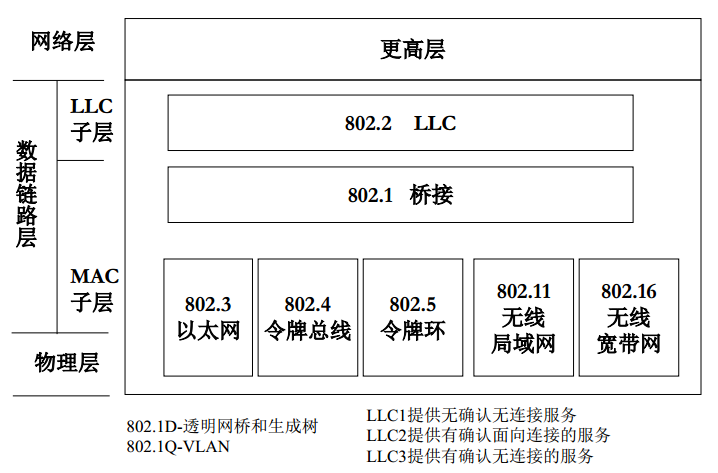
\includegraphics[width=0.65\linewidth]{fig/ieee802.PNG}
	\caption*{IEEE802系列标准}
\end{figure}

\subsection{逻辑链路控制子层}
\subsubsection{差错检测}
\begin{enumerate}
\item 奇偶校验:若接收方收到奇数个1,则有出错
\begin{itemize}
	\item 一维偶校验:只能检错;最后补一位使得全部为偶数个1,如$010$补为$010\mid 1$,而$101$补为$101\mid 0$
	\item 二维偶校验:检错+纠错一位;横纵同时偶校验
\end{itemize}
\item 校验和(checksum):将所有数据加起来,\textemph{每16位1组},最高位进位则\textemph{末尾加1},最后结果\textemph{取反}\\
由于需要使用加法器,校验和一般不用于数据链路层,而用在更高层(\textemph{网络层和传输层})
\begin{figure}[H]
	\centering
	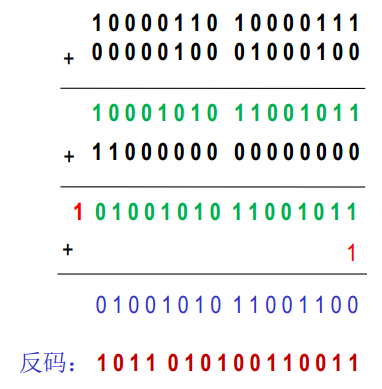
\includegraphics[width=0.3\linewidth]{fig/checksum.PNG}
\end{figure}
\item 循环冗余校验码(Cyclic Redundancy Check, CRC):
补充n位0后除以一个n+1位的除数,\textemph{模2除法}(\textemph{按位异或},做减法时没有借位);
如果传输过程中没有出现比特错,接收方用相同的除数去除[数据和CRC校验码],余数应该为0。
如下图,4位除数补3个0,最后的余数011即为校验码
\begin{figure}[H]
	\centering
	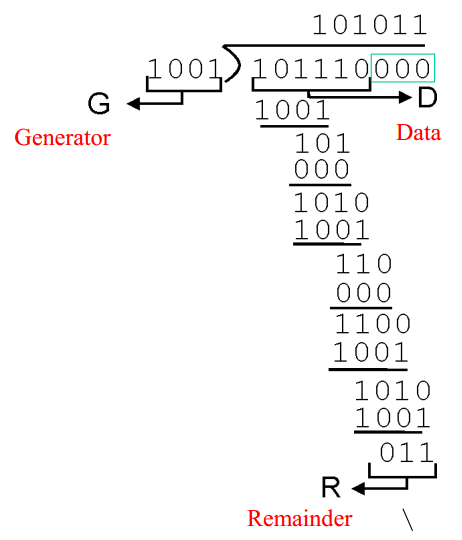
\includegraphics[width=0.3\linewidth]{fig/CRC.PNG}
\end{figure}
数据链路层采用\textemph{CRC-32}校验码,因为检错率很高,且容易实现(触发器+异或门)
\[x^{{32}}+x^{{26}}+x^{{23}}+x^{{22}}+x^{{16}}+x^{{12}}+x^{{11}}+x^{{10}}+x^{8}+x^{7}+x^{5}+x^{4}+x^{2}+x+1\]
\end{enumerate}

\subsubsection{差错控制}
流控制允许两个基站以不同的速率进行交互,主要有两大类方法:
\begin{enumerate}
	\item 基于反馈(feedback)的流控制:发送方要收到接收方返回的确认才执行下一步操作
	\item 基于速率(rate)的流控制:不需要接收方的确认,常被用于网络层和传输层
\end{enumerate}
数据链路层的流控制是\textemph{基于反馈}的,确认帧的返回限制了这段时间内发送方能够发送的帧的数目。
% https://www.tutorialspoint.com/flow-control-in-data-link-layer

每发送\textemph{一帧}都启动\textemph{一个超时定时器},如果它的确认帧(Acknowledgement frame, ACK)在其超时时间内到达就删除该定时器;否则,自动重发请求(Automatic Repeat reQuest, ARQ),重传该帧并重启定时器。

主要的ARQ协议包括\underline{停等协议}和\underline{滑动窗口协议}。

\myhline
\textbf{停等协议(stop-and-wait)}:只有收到前一个数据帧的确认帧才可以发送下一个数据帧,效率/吞吐量十分低,信道空闲时间长;最少需要\underline{2个序号}\footnote{数据帧丢失,则重新发送该帧即可;确认帧丢失或确认帧延迟都是对方已经收到数据帧,因而为了避免重复收取同一数据帧,就需要标号。
停等协议只需2个序号,0和1,轮流发送,如果重发则用同个序号,否则更换。
接收方通过序号的更换就可以确认上一个确认帧接收方已经收到。}。三种出错情况:
\begin{itemize}
	\item 数据帧丢失(loss):正向传递时丢包
	\item 确认帧丢失:回传时丢包
	\item 超时:收到ACK表明接收方一定收到,可以发送新的数据帧,重传的也一定要发ACK
\end{itemize}

\begin{example}
	把停等协议用于一个带宽为20Mbps、长度为3000公里、传播速度为200000公里/秒的点到点链路,如果最长帧为5000字节,带宽的最大利用率(最大吞吐量/带宽)是多少?
\end{example}
\begin{analysis}
	按照如下方法计算
	\begin{itemize}
		\item 传播延迟$RTT$:$(3\times 10^6 m) / (2\times 10^8 m/s)\times 2=30ms$(注意是\textemph{往返时间}!)
		\item 传输延迟$L/R$:$(5000B\times 8)/(20\times 10^6bps)=2ms$
		\item 吞吐量:$L/(RTT+L/R)=(5000B\times 8)/32ms=1.25Mbps$
		\item 带宽最大利用率:最大吞吐量/带宽=$1.25/20\times 100\%=6.25\%$
	\end{itemize}
	另,改为滑动窗口协议,窗口大小为8,则最大利用率为$8\times 6.25\%=50\%$
\end{analysis}

\myhline
\textbf{滑动窗口协议(sliding window)}:不需等待前面发送的帧的确认帧返回,就可以连续发送下一个,其个数不能超过发送窗口大小(sending window size, SWS)\footnote{SWS即连续发送数据帧可用序号范围,用于流控制:控制发送速度,否则会发生溢出(overlow),后面覆盖前面的}。

这里的确认帧是指\textemph{在此之前的帧都已全部收到并已交给上层协议}(直连网中间没有节点,后面收到前面一定收到;只要出错纠正不了直接丢弃),后面确认前面,提高可靠性。

滑动窗口协议又有以下两种:
\begin{itemize}
\item 回退N协议(go back N):某个ACK没收到则重传在此ACK之后的所有帧(超时重传)
\begin{figure}[H]
	\centering
	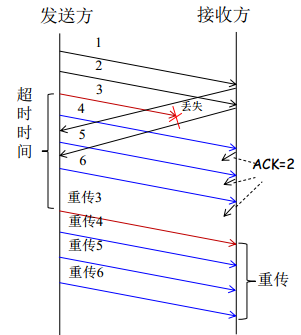
\includegraphics[width=0.3\linewidth]{fig/go-back-n.png}
\end{figure}
\begin{itemize}
	\item 发送窗口需要缓存SWS个帧,以便重传;发送窗口中序号最小的为sendBase;发送窗口之前的是已收到确认的,窗口内的是已发送但仍未收到确认的
	\item 回退N协议可能会\textemph{收到落在发送窗口之外的确认帧}:如果因确认帧迟到而出现超时重传,就可能收到一个帧的两个确认帧,第二个确认帧就会落在发送窗口之外
\end{itemize}
\item 选择性重传(selective repeat):通过发送否定性确认帧(negative acknowledgement, NAK)\footnote{如果不采用NAK,可以采用这样的方法:收到一个帧3个重复的确认帧后就重传该帧。这是网络层的实现方案,见后面的叙述。}要求重传该帧,每个帧只发送一次NAK
\begin{figure}[H]
	\centering
	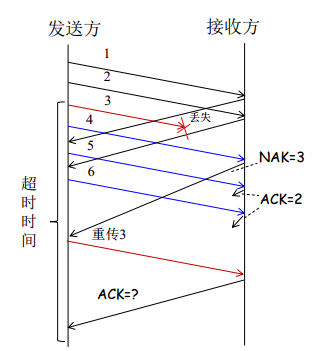
\includegraphics[width=0.3\linewidth]{fig/selective-repeat.png}
\end{figure}
\begin{itemize}
	\item 接收窗口(receiving window size, RWS)表示接收缓冲区大小(RWS$\leq$SWS,最好是等于,尽量减少重传帧;但序号少的话导致重复;错序到达的帧加上期待接收的帧最多SWS个),用于确定应该保存哪些帧,用序号范围表示,会存放错序到达的帧;其中最小序号帧是期待接受的帧(recvBase)
	\item 超时时间应略大约\textemph{2RTT}(否则会导致后续帧都重传\footnote{如果重置所有超时定时器,那超时时间可设为略大于1RTT});没有后续帧也会超时重传;无论窗口内窗口外收到都要发确认
	\item 选择性重传协议可能会\textemph{收到落在接收窗口之外的数据帧}:因确认帧丢失或超时到达而重传的数据帧都会落在接收窗口之外
	\item 选择性重传协议丢失了NAK并非致命错误,因为还有超时重传机制,保证该数据帧能够重新发送
\end{itemize}
\end{itemize}

ARQ协议的超时时间不应设置得太长,否则会导致系统需要花很长的时间来\underline{纠正这些错误,吞吐量低};但也不能设太短,否则发送方会\underline{大量误认为帧丢失}而产生不必要重传。

% 注意不管哪一种重传机制,序号都可以重复使用,因此有最小序号问题。

\begin{example}
	序号8个(0-7),SWS=RWS=4,按3456701234依次发送,RTT大于4帧的发送时间。第一个5丢失,包含重传帧在内的其它帧均正确到达接收方,问接收方依次收到这些帧(含重传帧)的序号
\end{example}
\begin{analysis}
	回退N:3467056701234
	\begin{center}
		\begin{tabular}{|c|c|c|}\hline
			SendWin & ReceWin & 操作\\\hline
			56 & X6 & 发ACK=4\\\hline
			5670 & X670 & 发ACK=4,重传整个发送窗口\\\hline
			(5670) & (5670) & 重传帧到达\\\hline
		\end{tabular}
	\end{center}
	选择性重传:3467051234
	\begin{center}
		\begin{tabular}{|c|c|c|}\hline
			SendWin & ReceWin & 操作\\\hline
			56 & X6 & 发NAK=5\\\hline
			5670 & X670 & 因NAK还没到达,发ACK=4\\\hline
			(5)670 & 670(5) & 重传5,要发回ACK=5,否则发送窗口动不了\\\hline
			1234 & 1234 & 发送窗口右移\\\hline
		\end{tabular}
	\end{center}
\end{analysis}

\myhline
提高滑动窗口协议的效率:
\begin{itemize}
	\item 选择性确认(selective acknowledgement):接受方把已收到的帧的序号告诉发送方,发送方要重传帧时,不会发送这些帧
	\item 捎带确认(piggybacking):通信双方\textemph{全双工}方式工作,接收方在发数据给对方时顺便把确认号也告诉对方(两个滑动窗口,两边都要发数据),需要结合延迟确认一起使用
	\item 延迟确认(delayed acknowledgement):接收方收到一帧后并不立即发送确认帧,而是等待一段时间再发送
\end{itemize}

\subsection{介质访问控制子层}
\subsubsection{简介}
\begin{enumerate}
\item \underline{PPP协议(point-to-point protocol):点到点网络}
\begin{itemize}
	\item 根据HDLC(high-level data link control)协议进行设计,
	主要用于串行电缆、电话线(MODEM)等串行链路
	\item 提供连接认证、传输加密和压缩功能,为网络层协议提供服务
	\item 采用\underline{字节填充法(byte-stuffing)}替换掉保留字
	\item \textemph{没有纠错}功能,也\textemph{没有流控制和确保有序}的功能
	\item ADSL的PPPoE和VPN中的PPTP协议都采用PPP协议进行封装
	\begin{figure}[H]
		\centering
		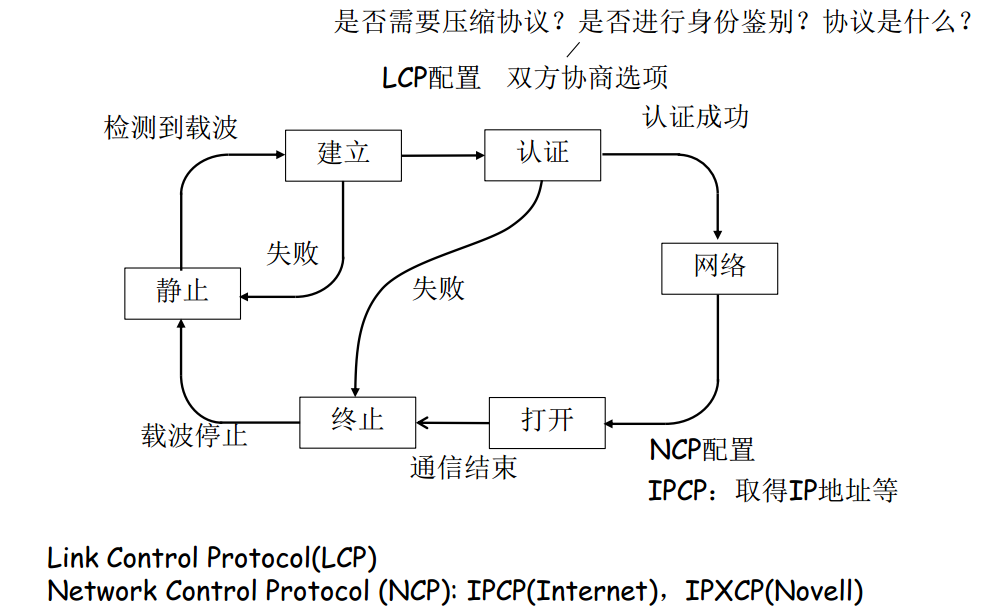
\includegraphics[width=0.6\linewidth]{fig/PPP.PNG}
	\end{figure}
\end{itemize}
\begin{center}
PPP协议数据帧格式\\
\begin{tabular}{|c|c|c|c|c|c|c|}\hline
1B & 1B & 1B & 1B-2B & $\leq$1500B & 2B-4B & 1B\\\hline
标志 & 地址 & 控制 & 协议 & 数据 & 校验码 & 标志\\\hline
0x7E & 0xFF & 0x03 & 0x0021 IP & $\cdots$ & CRC-16/CRC-32 & 0x7E\\\hline
\end{tabular}
\end{center}

\item \underline{以太网:多路访问网络},采用共享介质连接所有站点\\
解决冲突问题:\underline{随机访问协议}(random access protocol),注意不是滑动窗口\textemph{不用发确认帧}
\begin{itemize}
\item 纯ALOHA:想发送就发送,超时未收到确认则发生冲突
\item 分槽ALOHA:将时间分为长度相同的时槽,每个站点只在时槽开始时发送。\\
信道空,立即以概率$p$发送,以概率$1-p$延迟一个时间槽;信道忙,延迟一个时间槽。
\item 载波监听CSMA(Carrier Sense Multiple Access):发送前先监听信道
\begin{itemize}
	\item 信道空,立即发送;信道忙,持续监听(1-persistent CSMA,\textemph{以太网})
	\item 信道空,发送;信道忙,延迟一段随机长度时间(non-persistent CSMA,较省电)
	\item 信道空,立即以概率$p$发送,以概率$1-p$延迟一个时间槽;信道忙,延迟一个时间槽(p-persistent CSMA,\textemph{分槽ALOHA})
\end{itemize}
\end{itemize}
\end{enumerate}

\subsubsection{以太网物理层协议}
IEEE 802.3规定以太网物理层标准:
\begin{itemize}
	\item 传输方法:均使用\textemph{异步传输},即信道空闲时以太网设备不任何发送信号
	\item 编码方法:\textemph{曼彻斯特编码}
	\item 命名规则: 10BaseT的10表示10Mbps,Base表示基带传输,T表示双绞线;10Base2的2表示最大距离200m
\end{itemize}

\myhline
其他几种以太网(IEEE 802.3),主要是在\textemph{物理层}不同。
\begin{itemize}
\item 快速以太网(802.3u):只是把传输速率提高到100Mbps,其他均不变
\begin{itemize}
	\item MAC子层的协议不变:CSMA/CD协议不变,帧格式不变
	\item 最大距离改为100m (10base5的最大距离为2500m),物理层改动
	\item 帧间空隙隔依然为96b,即$0.96\mu s$
	\item 100Base-TX、100Base-T4、100Base-FX
\end{itemize}
\item 千兆以太网(802.3ab):除了把传输速率提高1000Mbps,其它不变
\item 万兆以太网
\begin{itemize}
	\item 保持帧格式不变
	\item 光纤或双绞线,全双工
	\item 无冲突,不使用CSMA/CD算法
\end{itemize}
\end{itemize}

\subsubsection{以太网MAC层协议}
以太网采用\underline{帧间空隙(interframe space)}的成帧方法(每帧发送前要求信道空闲时间至少为96bits,造成帧与帧之间有空隙)。
采用\underline{载波监听CSMA/CD(with collision detection)协议(1-坚持CSMA)}。
\begin{enumerate}
	\item 发送数据帧之前先\textemph{监听信道}。如果信道空闲,\textemph{立即}发送。
	如果信道忙,则\textemph{持续监听},直到信道空闲,立即发送。
	\item \textemph{边发送边检测}冲突。如果发送完毕都没有检测到冲突,则发送成功。
	\item 如果检测到冲突,则\textemph{停止发送},并发送32位干扰位(jamming signal)以加强冲突信号。
	采用二进制指数退避算法\textemph{随机延迟}一段时间后,转(1)。
\end{enumerate}

\myhline
\textbf{二进制指数退避算法}(binary exponential backoff)
\begin{itemize}
	\item 规定最短帧是为了使发送站点可以监测到所有冲突。
	选择\textemph{最短帧的发送时间}作为其时间槽(time slot)$\tau$的长度,其保证了首先发送的站点的信号可以到达最远的站点。
	如果先发送的只有一个站点,其他站点要不就检测到发送站点的信号而不能发送,要不就因为发送站点发送完毕而检测到信道空闲,总之不会产生过冲突。
	即任何间隔$\tau$或以上时间的两个发送数据的站点不会发生冲突。
	\item 时间片$\tau$的长度为512b时间,10Mbps的以太网为51.2$\mu s$
	\item 第$i$次冲突从$0,1,\ldots,2^j-1$个时间片随机选择一个,$i<16$,$j = min(i,10)$
	\item 前十次冲突后\textemph{可选时间片数量每次加倍},后五次冲突后\textemph{可选时间片数量不变},\\
	所以也称为截止式(truncated)二进制指数退避算法
\end{itemize}

\begin{example}
	当一个以太网的信道忙时有五个站点都想发送一个最长帧(长度为1520B),如果很长时间只有这五帧要发送,问最少经过几次冲突就可以全部发送成功?
\end{example}
\begin{analysis}
	最长帧占用$1520B\times 8/512b=23.75$个时间槽,而在第1、2、3、4次冲突的延迟时间最多16个时间槽,首先发送的站点都会引起后续所有站点冲突。
	最好情况每次冲突后都让一个站点发送成功,所以最少4次冲突。
	详细来说,一开始5个站点同时发送,第一次冲突,随机延迟0或1个时间片,假设0号立即发送,其他4个延后1个时间片,那么0号发送成功,其他4个检测到信道忙,不发送。
	到0号发完时,信道空闲,其他4个同时发送,第二次冲突,如此类推,每次成功发送一个。
\end{analysis}

\myhline
\textbf{802.3的MAC帧格式}
\begin{center}
\begin{tabular}{|c|c|c|c|c|c|}\hline
8B & 6B & 6B & 2B & 46B-1500B & 4B\\\hline
前导字符 & 目的地址 & 源地址 & 类型/长度 & 有效载荷/填充位\protect\footnote{这实际上决定了最小和最大传输单元(Maximum Transmission Unit, MTU),为什么定这两个值可以见\url{https://community.cisco.com/t5/other-network-architecture/why-the-mtu-size-is-1500/td-p/105418}} & 帧校验序列\\\hline
\end{tabular}
\end{center}
\begin{itemize}
\item 前导字符(preamble):同步字符(7B)和起始定界符(start of frame delimiter)(1B)
\item 目的地址:可以为接受者的单播、多播或广播地址
\item 源地址:一般为发送者的单播地址
\item 类型/长度:\textemph{0x0800 IP数据报,0x0806 ARP报文},0x0835 RARP报文
\item 有效载荷(payload):用户数据,不足46B加入填充字节至46B
\item 帧校验序列(frame check sequence):对\underline{目的地址、源地址、类型/长度、有效载荷、填充位}进行\textemph{CRC-32}校验
\end{itemize}

\myhline
\textbf{接收帧的方法}
\begin{enumerate}
	\item 以太网站点(网卡)会缓存所有的帧
	\item 如果缓存的帧有错(长度错误,CRC错等),则\textemph{丢弃}它。
	\item 如果缓存的帧的目的地址为单播地址并且与接收该帧的网卡的MAC地址一致,则接收它。
	如果目的地址为多播地址并且为网卡预设的多播地址之一,或者为广播地址,也接收它。
	其它情况则丢弃它。
	\item 如果把网卡设置为\underline{混杂模式}则会接收所有无错的帧。
\end{enumerate}

\subsubsection{令牌环网}
令牌环网(token ring, IEEE 802.5)通过在站点之间传递令牌防止冲突并且具有\textemph{优先权}的星形\textemph{LAN},为\underline{轮流协议}(take turns protocol),要与以太网的\underline{随机访问协议}区分。

多站点接入部件称为MSAU(multistation access unit)
\begin{figure}[H]
	\centering
	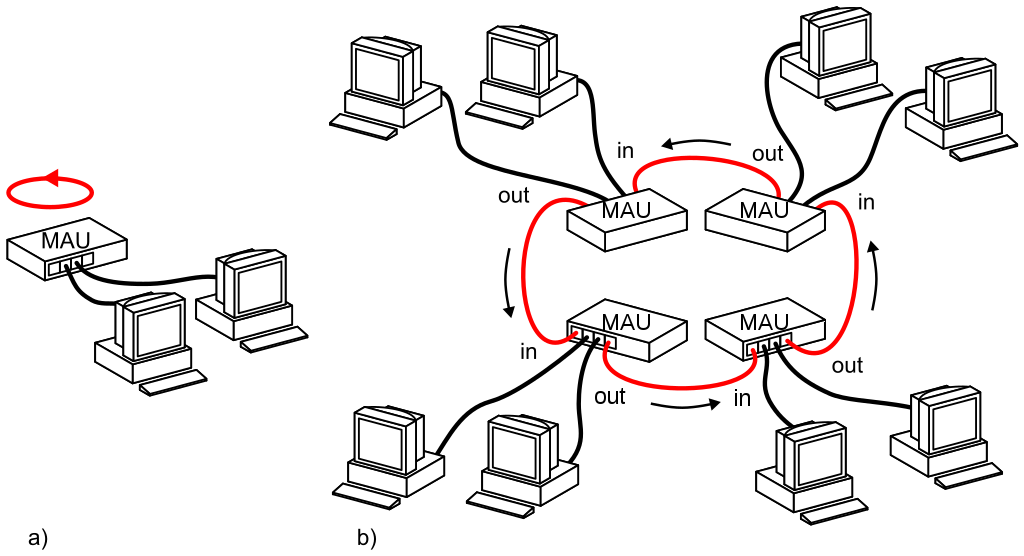
\includegraphics[width=0.5\linewidth]{fig/token-ring.png}
\end{figure}

数据传送过程:
\begin{itemize}
	\item 令牌(帧)绕环而行
	\item 只有截获令牌的站点才可以发送数据帧,各站点保有令牌帧的时间是相同的
	\item 发送的数据帧通过所有的活动站点
	\item 目的站点拷贝数据帧
	\item 只有发送方移除数据帧
	\item 当没有数据帧要发送或者持有时间到,当前的发送站点要释放令牌;被释放的令牌继续绕环而行
\end{itemize}

注意:\textemph{以太网没有确认机制,没有优先权。}
令牌环网必然有特殊的站点(监控站点)产生令牌帧,选举出监控站点(MAC地址最小)。

光纤分布式数据接口(Fiber Distributed Data Interface, FDDI)是另一种采用了令牌环的局域网,是一种100 Mbps的光纤局域网。

源路由桥接算法:由IBM开发的用于令牌环网的协议,将路径记到头部,下一次就不用查。
为了兼容普通交换机,源路由网桥交换机也必须实现透明网桥的功能。

\subsection{透明网桥}
用网桥(bridge)连接若干局域网(LAN)可以建造一个更大的局域网, 称为桥接局域网(bridged LAN)或\\\underline{扩展局域网}(extended LAN)。
原来的局域网就成为该扩展局域网的一部分,称为该扩展局域网的一个网段(segment)。
\begin{figure}[H]
	\centering
	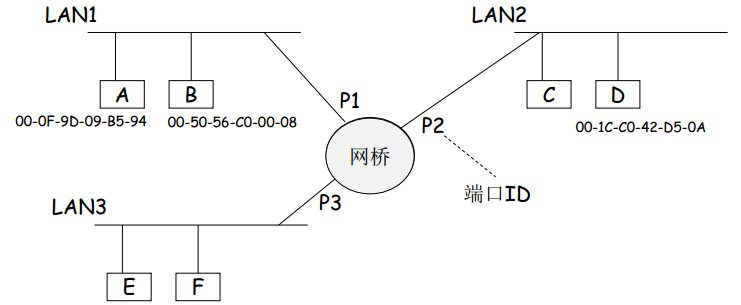
\includegraphics[width=0.6\linewidth]{fig/extended-LAN.png}
\end{figure}

透明网桥的三个操作:
\begin{itemize}
	\item 表里查到则\underline{\textemph{转发}}(forward)
	\item 表里没有则\underline{\textemph{扩散/泛洪}}(flood)
	\item 从某一条路发来则不能传回去,过滤/\underline{\textemph{丢弃}}(filter)
\end{itemize}

透明网桥有自学习机制:利用\textemph{源地址}学习,如信息从A主机-P1端口来,则记为A-P1,同时设好生存期(Time to live, TTL)\footnote{单位为秒,每次发送都会重置,对于不活跃的表项自动删掉(减少表的大小,查找速度更快)}。
如果收到的帧有错则直接丢弃,根本不会学习。
如果源地址已经在表中,则更新记录,并\textemph{重置超时计时器}。

之所以称为透明,是因为插入网桥后无需改动硬件和软件,也无需设置地址开关、装入路由表或参数等,网桥就能工作(自学习)。

\begin{example}
	下面的扩展LAN包含三个透明网桥B1、B2、B3和四台主机A、C、D、E。
	如果网桥的MAC地址表初始都是空的,在以下三次传输之后MAC地址表的内容是什么?
	\begin{enumerate}
	\item D发送了一个帧给E
	\item A发送了一个帧给D
	\item C发送了一个帧给A
	\end{enumerate}
	\begin{figure}[H]
		\centering
		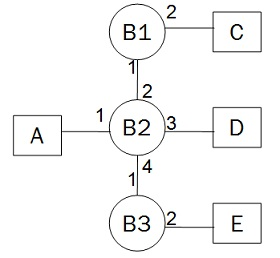
\includegraphics[width=0.25\linewidth]{fig/mac_address.jpg}
	\end{figure}
\end{example}
\begin{analysis}
	MAC地址表如下
	\begin{center}
		\begin{tabular}{cc|cc|cc}\hline
			B1 MAC地址 & 端口 & B2 MAC地址 & 端口 & B3 MAC地址 & 端口\\\hline
			D & 1 & D & 3 & D & 1\\
			C & 2 & A & 1 & & \\
			& & C & 2 & & \\\hline
		\end{tabular}
	\end{center}
\end{analysis}

\subsection{生成树协议}
生成树协议(spanning tree protocol, STP)将所有的LAN和网桥都抽象为结点,避免冲突即构造一棵生成树(注意不是最小生成树)
\begin{itemize}
\item IEEE 802.1D 生成树协议+透明网桥
\item IEEE 802.1w RSTP(Rapid Spanning Tree Protocol)
\end{itemize}

工作流程如下
\begin{itemize}
\item 先确定\underline{根网桥},即\textemph{网桥ID(Bridge ID, BID)最小}的
\item 每个网段(需要集线器)依赖于连通的网桥,每个网桥都把\textemph{自己到根的距离}发出去(竞选/配置消息)
\item 网桥之间的开销为1,选一条\textemph{最短路径}
\item 扩散自己BID,最后只剩下根网桥认为自己是根。
取得优胜的,作为\underline{指定网桥}(网段上离根最近的网桥);相同距离时,BID小的优胜;相同BID,端口号小的优胜
\item \textemph{网桥}上离根最近的端口为\underline{根端口},指定网桥上与网段相连的端口为\underline{指定端口},网桥上非根端口又非指定端口的为\underline{阻塞端口}
\item 网桥只在根端口和指定端口之间转发数据帧,不可通过阻塞端口
\item 只有\textemph{从根端口过来}的才扩散配置消息,其他端口来的不扩散,这样不会形成回路
\item 断了/失效了则变成无穷大,其他网桥可成为指定网桥
\end{itemize}

生成树协议既能防止广播风暴,又能自动修复损害网桥(通过冗余方式),增加可靠性
\begin{example}
	下图显示了由五个透明网桥(B1-B5)形成的扩展LAN,A-D为网段。
	\begin{figure}[H]
		\centering
		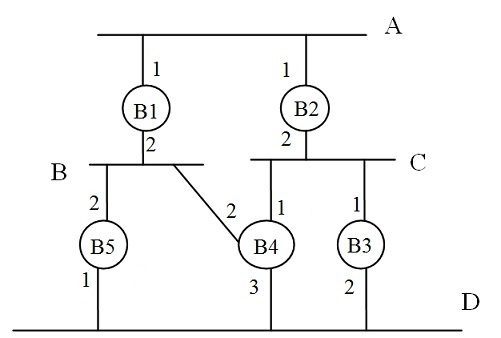
\includegraphics[width=0.4\linewidth]{fig/bridge.jpg}
	\end{figure}
\end{example}
\begin{analysis}
\begin{enumerate}
	\item B1是根网桥
	\item 网段A-D的指定网桥(designated bridges)分别是
\begin{center}
	\begin{tabular}{|c|c|c|c|c|}\hline
		 & A & B & C & D\\\hline
		指定网桥 & B1 & B1 & B2 & B4\\\hline
	\end{tabular}
\end{center}
\item 网桥B1-B5的根端口、指定端口和阻塞端口分别是
\begin{center}
	\begin{tabular}{|c|c|c|c|c|c|}\hline
		& B1 & B2 & B3 & B4 & B5\\\hline
		根端口 & 无 & 1 & 1 & 2 & 2\\\hline
		指定端口 & 1,2 & 2 & 无 & 3 & 无\\\hline
		阻塞端口 & 无 & 无 & 2 & 1 & 1\\\hline
	\end{tabular}
\end{center}
\end{enumerate}
\end{analysis}

\begin{example}
	下图是一个扩展LAN:
	\begin{figure}[H]
		\centering
		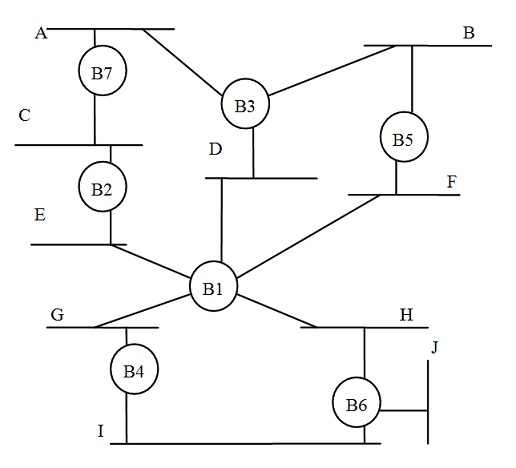
\includegraphics[width=0.4\linewidth]{fig/spanning_tree.jpg}
	\end{figure}
\end{example}
\begin{analysis}
	\begin{itemize}
		\item[a.] 如果B1没有启动生成树算法但是转发生成树消息(BPDU),只生成1棵生成树,根为B2
		\item[b.] 如果B1没有启动生成树算法而且丢弃所有收到的生成树消息(BPDU),
		生成2棵生成树,根分别为B2和B4
	\end{itemize}
\end{analysis}

\subsection{虚拟局域网}
虚拟局域网(Virtual LAN, VLAN, IEEE 802.1Q)将原来的局域网分割成多个相互隔离的局域网,只在具有相同标号(VLAN ID)的端口间转发。

如果所有交换机都是连通的,并且交换机连至交换机的接口都配置为干道(trunk)接口,交换机连至主机的接口都配置为VLAN接口(主机接口),则所有连至相同的VLAN接口的主机都位于\textemph{同一个广播域},连至不同VLAN接口的主机位于不同的广播域。

每次扩散到帧内指定的端口或\textemph{干道端口},同样查MAC地址表转发。
只有发往干道端口的帧才需要\textemph{加上VLAN ID}。
如果从干道收到的帧没有VLAN ID,则认为是本征(native)VLAN,默认为VLAN 1。
\begin{example}
	下图中哪些发送的帧将被目的主机收到
	\begin{figure}[H]
		\centering
		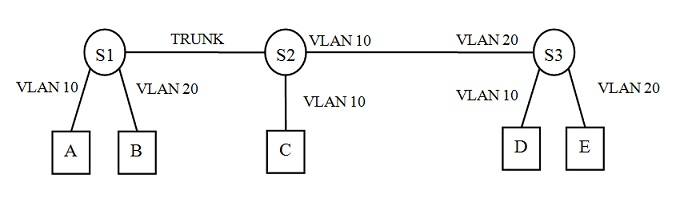
\includegraphics[width=0.6\linewidth]{fig/vlan.jpg}
	\end{figure}
\end{example}
\begin{analysis}
	只有A到E或E到A可以成功发送信息,注意S2和S3的端口设错了(故意的)。
	如E到A,VLAN20经过S3转发到VLAN20,发到S2。
	S2误认为是从VLAN10发来的消息,故扩散到干道端口TRUNK加VLAN10,发到S1。
	S1接收到后转发至VLAN10。\\
	而D到B没有办法,因为从S3就转发不出去,没有干道端口。
\end{analysis}

\begin{center}
	\textbf{虚拟局域网帧格式}\\
	\begin{tabular}{|c|c|c|c|c|c|c|}\hline
		6B & 6B & 2B & 2B & 2B & 46B-1500B & 4B\\\hline
		目的地址 & 源地址 & 协议(\verb'0x8100') & \begin{tabular}{l}3b 优先权\\1b 标准格式指示位\\12b VLAN ID\end{tabular} & 类型 & 数据 & CRC-32\\\hline
	\end{tabular}
\end{center}

多生成树协议:管理员规定哪些VLAN为一组,构成多生成树,其余的用公共生成树
\begin{itemize}
	\item 公共生成树(common spanning tree, CST)
	\item 多生成树(Multiple spanning tree protocol, MSTP)
\end{itemize}

\subsection{物理设备}
集线器(hub)属于物理层的器件,采用电子线路方法模拟总线方式的以太网,若两台主机同时发送会产生冲突,所以是\textemph{半双工}工作。
如果通过两个接口同时发送数据会产生冲突,则这两个接口属于同一个\underline{冲突域}(collision domain)。

一个广播帧可以到达的所有接口属于同一个\underline{广播域}。
属于同一个冲突域的以太网部分称为\underline{网段}(segment)。
\begin{example}
	下图的冲突域和广播域个数?
	\begin{figure}[H]
		\centering
		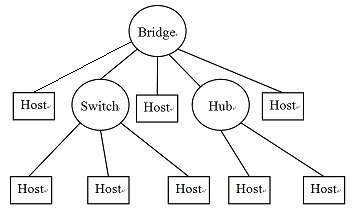
\includegraphics[width=0.35\linewidth]{fig/conflict_count.jpg}
	\end{figure}
\end{example}
\begin{analysis}
交换机(switch)/网桥(bridge)的\textemph{每个端口处于一个冲突域},集线器(hub)的\textemph{所有端口处于一个冲突域}。
故8个冲突域,1个广播域。
\end{analysis}

\myhline
交换机(switch)是一个把多个网段连接起来的设备,也称为\textemph{多端口网桥}。
\begin{figure}[H]
	\centering
	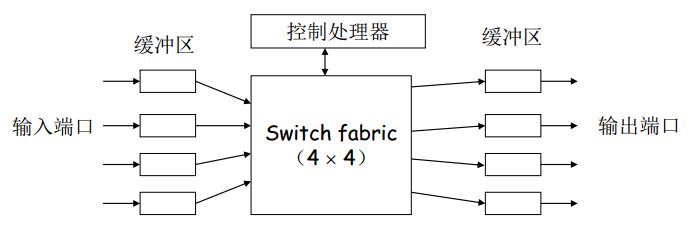
\includegraphics[width=0.6\linewidth]{fig/switch.png}
\end{figure}

\myhline
交换结构(fabrics)
\begin{itemize}
	\item 共享总线式:存在冲突问题
	\begin{figure}[H]
		\centering
		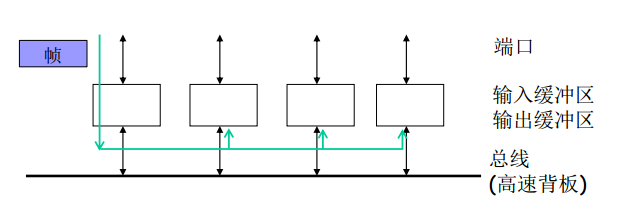
\includegraphics[width=0.6\linewidth]{fig/switch-share.png}
	\end{figure}
	\item 纵横式(crossbar):可实现多路并行传输
	\begin{figure}[H]
		\centering
		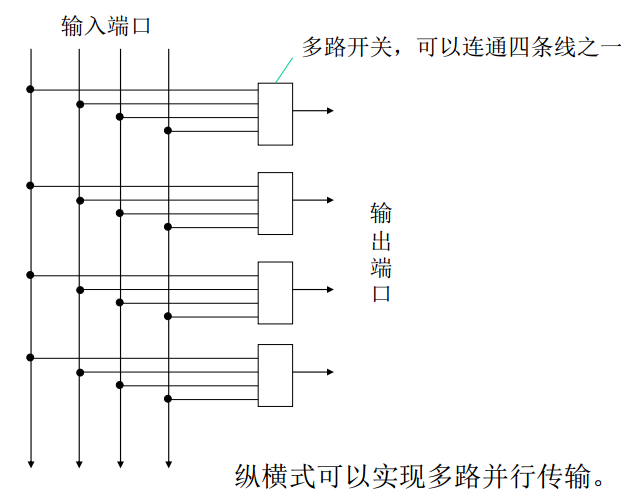
\includegraphics[width=0.5\linewidth]{fig/switch-crossbar.png}
	\end{figure}
\end{itemize}

\myhline
交换机转发方法
\begin{itemize}
\item 存储转发(store and forward):交换机收到\textemph{整个帧}后转发,大多数采用该模式,转也要依照CSMA/CD来转发
\item 直通(cut through):收到帧的\textemph{硬件地址}后立即转发它,出现碎片
\item 无碎片(fragment free):交换机不用收到整个帧而是收到\textemph{64B(冲突窗口,最小帧保证})后,都没冲突才开始转发
\item 适应性交换(adaptive switching):自动在上面三种方式中选择
\end{itemize}

\myhline
交换机的工作模式
\begin{itemize}
\item 全双工模式:因为没有冲突,CSMA/CD算法可以被关闭
\item 自动翻转(auto-MDIX):
大部分交换机可以自动选择连接方式,\textemph{交叉线}或\textemph{直通线}
\begin{figure}[H]
	\centering
	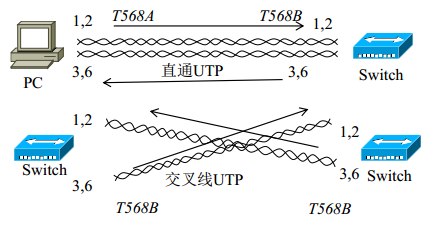
\includegraphics[width=0.5\linewidth]{fig/auto-MDIX.png}
\end{figure}
\item 自适应(autonegotiation):两个站点周期性使用快速链路脉冲(fast link pulse,FLP),\\
选择10M/100M/1000Mbps自适应
\end{itemize}

\myhline
集线器、交换机、路由器的区别如下\footnote{\url{http://www.qianjia.com/html/2017-08/09_274208.html}}:
\begin{itemize}
	\item 集线器(hub):\textemph{物理层/一层},广播,排队,冲突,共享型设备(一个端口往另一个端口发数据,其他端口就处于等待状态,全部端口属于一个冲突域),半双工,监听,响应
	\item 交换机(switch):\textemph{数据链路层/二层},MAC地址,建立连接,独享信道,全双工,\\\underline{增加冲突域数量,减少冲突范围大小}
	\item 路由器(router):\textemph{网络层/三层},建立路由表,IP地址,路由选择
\end{itemize}

路由器能连接\textemph{不同类型的网络},如以太网、ATM网、FDDI网、令牌环网等,并实现\textemph{帧类型的转换},但集线器和交换机一般只用于连接以太网。

小范围的局域网,如我们的校园网大多采用交换机,路由器少。

注意交换机\textemph{相当于\textcolor{red}{透明}网桥},故路由器不会知道,路由器只知道下一跳。